\documentclass[a4paper, 11pt, normalem]{report}

\usepackage{../../../LaTeX-Templates/Notes}
\usepackage{subfiles}
\usetikzlibrary{arrows.meta}

\newcommand\xo{\hat{X}_1}
\newcommand\xt{\hat{X}_2}
\newcommand\hsig{\hat{\sigma}}
\newcommand\hd{\hat{\unl{d}}}

\title{Advanced Theoretical Physics \vspace{-20pt}}
\author{Dr Kendon and Prof Gardiner}
\date{\vspace{-15pt}Michaelmas Term 2019 - Epiphany Term 2020}
\rhead{\hyperlink{page.1}{Contents}}

\begin{document}

\maketitle
\tableofcontents

\part{Quantum Optics}
\chapter{}
\textbf{Syllabus:}
\begin{multicols}{2}
\begin{itemize}
    \item quantization of light
    \item creation and annihilation operators
    \item Hamiltonian of the E field
    \item number states
    \item coherent states
    \item squeezed states
    \item photon bunching and anti-bunching
    \item density operator
    \item pure states, mixed sates, entangled states
    \item decoherence
    \item atom-light interactions
    \item applications
\end{itemize}
\end{multicols}

\begin{figure}[H]
    \centering
    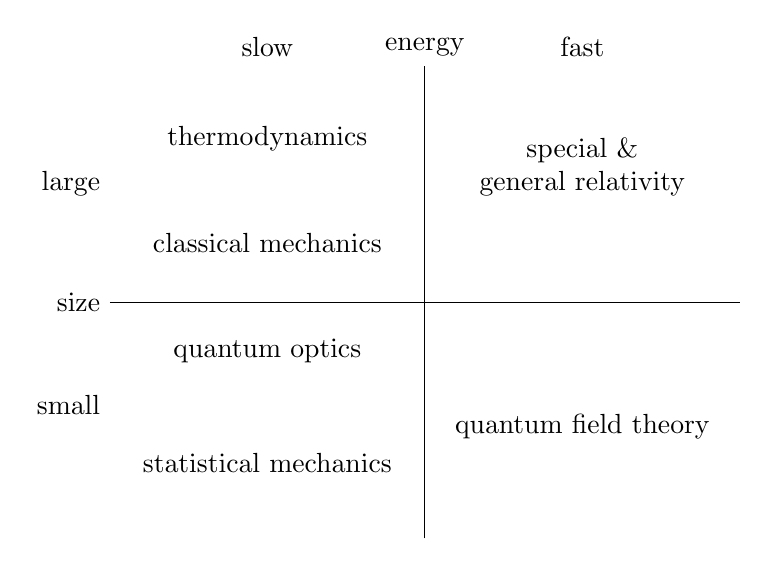
\begin{tikzpicture}
        \draw (-4,0) node[anchor=east] {size} -- (4,0);
        \draw (0,-3) -- (0,3) node[anchor=south] {energy};
        \draw[white] (-2.1,3) -- (-1.9,3) node[black,midway,anchor=south] {slow};
        \draw[white] (1.9,3) -- (2.1,3) node[black,midway,anchor=south] {fast};
        \draw[white] (-4,1.5) node[black,anchor=east] {large} -- (-3.9,1.5);
        \draw[white] (-4,-1.3) node[black,anchor=east] {small} -- (-3.9,-1.3);
        \draw[white] (-2.1,-0.35) -- (-1.9,-0.35) node[black,midway,anchor=north,align=center] {quantum optics};
        \draw[white] (-2.1,-1.8) -- (-1.9,-1.8) node[black,midway,anchor=north,align=center] {statistical mechanics};
        \draw[white] (-2.1,1.8) -- (-1.9,1.8) node[black,midway,anchor=south,align=center] {thermodynamics};
        \draw[white] (1.9,2.2) -- (2.1,2.2) node[black,midway,anchor=north,align=center] {\shortstack{special \&\\general relativity}};
        \draw[white] (1.9,-1.3) -- (2.1,-1.3) node[black,midway,anchor=north,align=center] {quantum field theory};
        \draw[white] (-2.1,0.5) -- (-1.9,0.5) node[black,midway,anchor=south,align=center] {classical mechanics};
    \end{tikzpicture}
\end{figure}

\textbf{Ingredients:}
\begin{itemize}
    \item harmonic oscillators
    \item Gaussian integrals
    \item Hamiltonian mechanics (canonical variables q and p)
    \item maths of operators - adjoint, self-adjoint, Hermitian, commutation relations
    \item QM in both Schrodinger and Heisenberg pictures
    \item density matrices
    \item classical EM - Maxwell's equations in Coulomb gauge - especially plane waves and dipoles
\end{itemize}

Hanbury Brown and Tiss:
\begin{equation}
    G(\tau) = I_A(t)I_B(t+\tau)
\end{equation}

\chapter{}
\section{Learning Outcomes}
To be able to state, explain and apply the operator formalism of the quantum harmonic oscillator, including:
\begin{itemize}
    \item the Hamiltonian in terms of the creation and annihilation operators
    \item the number operator and number states, eigenstates of the Hamiltonian
    \item definition of the creation and annihilation operators, commutation relations, adjoint and self-adjoint operators
    \item mathematical properties of the number states, completeness
    \item systems of two or more independent oscillators
\end{itemize}


\section{Quantum Harmonic Oscillator}
\begin{align}
    F &= ma = m\ddot{x} \\
      &= -kx \\
    x(t) &= x_0\sin\om t \\
    p_x(t) &= p_0\cos\om t \\
    V(x) &= \frac12 kx^2 = \frac12 m\om^2x^2 \\
    \frac{\hbar^2}{2m}\frac{d^2\psi}{dx^2} &+ V(x)\psi(x) = E\psi \\
    E_n &= \left(n+\frac12\right)\hbar\om
\end{align}
   
\begin{figure}[H]
    \centering
    \begin{tikzpicture}
        \draw[->,thick] (-3,0) -- (3,0) node[anchor=south] {$x$};
        \draw[->,thick] (0,-0.3) -- (0,2) node[anchor=south] {$V(x)$};
        \draw (0,0) parabola (2.5,1.8);
        \draw (0,0) parabola (-2.5,1.8);
    \end{tikzpicture}
\end{figure}
Start with writing the Hamiltonian, then turn everything into operators
\begin{align}
    H &= \frac{p^2}{2m} + \underbrace{\frac12 m\om^2x^2}_{V(x)} \\
    p &\to \hp = -i\hbar\frac{d}{dx},~ x \to \hx \\
    [\hx,\hp] &= i\hbar \\
    H &= \frac{\hp^2}{2m} + \frac12m\om^2\hx^2 \\
    \ha &= \frac{1}{\sqrt{2m\hbar\om}}\left(m\om\hx+i\hp\right) \\
    \hag &= \frac{1}{\sqrt{2m\hbar\om}} \left(m\om\hx - i\hp\right) \\
    \hx &= \left(\frac{\hbar}{2m\om}\right)^{1/2}(\ha+\hag) \\
    \hp &= -i\left(\frac{m\hbar\om}{2}\right)^{1/2}(\ha-\hag) \\
    [\ha,\hag] &= \ha\hag - \hag\ha = 1 \\
    \hh &= \hbar\om(\hag\ha+\frac12) \\
    \hag\ha &= \hn,~ \hn|n\rangle = n|n\rangle \\
    \hh|n\rangle &= \hbar\om\left(n+\frac12\right)|n\rangle = E_n|n\rangle
\end{align}
How do the annihilation and creation operators, $\ha$ and $\hag$ interact with the number states, $|n\rangle$?
\begin{align}
    \hag|n\rangle &= \sqrt{n+1}|n+1\rangle \\
    \ha|n\rangle &= \sqrt{n}|n-1\rangle
\end{align}
Together, the creation and annihilation operators are known as the \textit{ladder operators.}
Ladder operators move the system up or down the energy levels of the harmonic potential.
\begin{figure}[H]
    \centering
    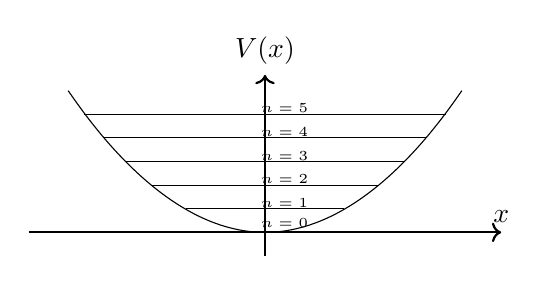
\begin{tikzpicture}
        \draw[->,thick] (-3,0) -- (3,0) node[anchor=south] {$x$} node[anchor=south,midway,xshift=7pt,yshift=-2pt] {\tiny $n=0$};
        \draw[->,thick] (0,-0.3) -- (0,2) node[anchor=south] {$V(x)$};
        \draw (0,0) parabola (2.5,1.8);
        \draw (0,0) parabola (-2.5,1.8);
        \draw (-2.3,1.5) -- (2.3,1.5) node[anchor=south,midway,xshift=7pt,yshift=-3pt] {\tiny $n=5$};
        \draw (-2.05,1.2) -- (2.05,1.2) node[anchor=south,midway,xshift=7pt,yshift=-3pt] {\tiny $n=4$};
        \draw (-1.78,0.9) -- (1.78,0.9) node[anchor=south,midway,xshift=7pt,yshift=-3pt] {\tiny $n=3$};
        \draw (-1.45,0.6) -- (1.45,0.6) node[anchor=south,midway,xshift=7pt,yshift=-3pt] {\tiny $n=2$};
        \draw (-1,0.3) -- (1,0.3) node[anchor=south,midway,xshift=7pt,yshift=-3pt] {\tiny $n=1$};
    \end{tikzpicture}
\end{figure}
We now have a partly new mathematical representation. 
Notice that the potential still remains positive, it does not go negative.
Therefore we must have:
\begin{align}
    \ha|0\rangle &= 0, \\
    \hn &= \hag\ha|0\rangle = 0. \\
    \implies \hh|0\rangle &= E_0|0\rangle = \frac12\hbar\om|0\rangle
\end{align}
So the ground state is labelled '0' but does not have $E=0$.\\
Now we introduce $\hog$ as the adjoint of $\ho$ if
\begin{align}
    \langle\psi|\ho|\phi\rangle &= \langle\phi|\hog|\psi\rangle^*\; \forall \psi,\phi
\end{align}
A self-adjoint operator is equivalent to a Hermitian operator, i.e. $\hn, \hh$.\\
For adjoint operators:
\begin{align}
    (\hat{A}+\hat{B})^\dagger &= \hat{A}^\dagger + \hat{B}^\dagger \\
    (\hat{A}\hat{B})^\dagger &= \hat{B}^\dagger\hat{A}^\dagger \\
    (c\hat{A})^\dagger &+ c^*\hat{A}^\dagger \\
    (\hat{A}^\dagger)^\dagger &= \hat{A}
\end{align}
More on the number states:
\begin{itemize}
    \item they are orthogonal
        \begin{align}
            \langle n|n\rangle &= 1 \\
            \langle n|m\rangle &= 0,~ n\neq m \\
            \langle n|m\rangle &= \delta_{n,m} \\
        \end{align}
    \item they form a basis (note: not mathematically a Hilbert space, but a Banah(?) space)
        \begin{align}
            |\psi\rangle &= \sum_n c_n|n\rangle \\
            0 &\leq n \leq \infty
        \end{align}
\end{itemize}

\section{Two Oscillators - independent}
\begin{align}
    |\psi_0\rangle &= \sum_n c_n|n\rangle_0 \\
    |\psi_1\rangle &= \sum_m c_m|m\rangle_1 \\
    |\psi_{01}\rangle &= \sum_{n,m} c_{n,m}|n\rangle_0|m\rangle_1
\end{align}
What we are doing is "tensoring" the Hilbert spaces: $\mathcal{H}_0 \otimes \mathcal{H}_1$:
\begin{align}
    |n\rangle_0|m\rangle_1 &\equiv |n\rangle_0\otimes|m\rangle_1.
\end{align}
Now we have the operators, $\ha_0,\hag_0,\ha_1,\hag_1$:
\begin{align}
    \ha_0 \otimes \mathbb{I}_1&,~ \mathbb{I}_0\otimes \ha_1,\dots \\
    [\ha_0,\ha_1] &= [\ha_0,\hag_1] = 0 \\
    \hh &= \hh_0\otimes\mathbb{I}_1 + \mathbb{I}_1\otimes\hh_1 
\end{align}
Note this is for non-interacting oscillators. 
For interacting, 
\begin{align}
    \hh &= \hh_0\otimes\mathbb{I}_1 + \mathbb{I}_1\otimes\hh_1 + \mathcal{H}_{int}.
\end{align}

\chapter{}
\section{Learning Outcomes}
To be familiar with the route to quantisation of the electromagnetic field, in particular to:
\begin{itemize}
    \item Explain and state the description of the electromagnetic field in terms of modes, including polarization
    \item Be familiar with the equivalence between a mode of the field and a quantum harmonic oscillator
    \item To explain the form of (but not derive) expressions for the Hamiltonian of the electromagnetic field, and the electric and magnetic fields in terms of the creation and annihilation operatoes
    \item To recognise and explain the concepts of the Schrodinger and Heisenberg representations, and to explain which is being applied
    \item To explain and apply the concepts of adjoint and self-adjoint operators and their matrix elements
\end{itemize}

\section{Quantising the EM field}
Consider an EM scalar potential, $\phi=0$ (no free charges), and a vector potential, $\unl{A}$.
\begin{align}
    \E(\vr,t) &= \frac{\p}{\p t}\unl{A} & \B(\vr,t) &= \del\times\unl{A}(\vr,t) \\
    \grad\left[\grad\cdot\unl{A}\right] &- \del^2\unl{A} + \frac{1}{c^2}\frac{\p^2}{\p t^2}\unl{A} = 0
\end{align}
Coulomb gauge, $\del\cdot\unl{A} = 0$.
\begin{align}
    \unl{A} &= \sum_{\unl{k}} \left\{ \unl{A}_{\unl{k}}\exp\left[i(\unl{k}\cdot\unl{r}-\om_kt)\right] + \unl{A}^*_{\unl{k}}\exp\left[-i(\unl{k}\cdot\unl{r} - \om_kt)\right]\right\} \\
    \om_k &= c|k|,~ \unl{k}\cdot\unl{A}_{k} = 0
\end{align}
Polarisation vectors, $\ve_{k1},\ve_{k2}$ - orthonormal vectors perpendicular to $\unl{k}$.
\begin{align}
    \unl{A}_k &= A_{k1}\ve_{k1} + A_{k2}\ve_{k2} \\
    \unl{A} &= \sum_{\unl{k},s} A_{\unl{k},s}\ve_{\unl{k},s}\exp\left\{i(\unl{k}\cdot\vr-\om_kt)\right\} + A_{\unl{k},s}^*\ve_{\unl{k},s}\exp\left\{-i(\unl{k}\cdot\vr-\om_kt)\right\}
\end{align}
The labels of the modes are $\unl{k},s$, $s\in1,2$. 
They gives us the: direction; wavelength, $\frac{2\pi}{|\unl{k}|}$; and polarisation, $s$.\\
To quantise this classically:
\begin{align}
    H &= \frac12\e_0 \int \left(\E\cdot\E + c^2\B\cdot\B\right)\,dV \\
      &= 2\e_0 V \sum_{\unl{k},s} \om_k^2 A_{\unl{k},s}A_{\unl{k},s}^* \\
    A_{\unl{k},s} &= \frac{1}{2\om_k\sqrt{\e_0V}} \left\{\om_kq_{\unl{k},s} + ip_{\unl{k},s}\right\} \\
    A_{\unl{k},s}^* &= \frac{1}{2\om_k\sqrt{\e_0V}} \left\{\om_kq_{\unl{k},s} - ip_{\unl{k},s}\right\}
\end{align}
$q_{\unl{k},s},p_{\unl{k},s}$ canonical coordinates $(x,p)$.
\begin{align}
    H_{\unl{k},s} &= \frac12\left(p^2_{\unl{k},s} + \om_k^2q_{\unl{k},s}\right)
\end{align}
Harmonic oscillator $m=1$, $x\leftrightarrow p$.
To transfer this from classical to quantum, you simply convert everything to its operator form. 
For a single mode:
\begin{align}
    \hh_{\unl{k},s} &= \left(\hag_{\unl{k},s}\ha_{\unl{k},s} + \frac12\right)\hbar\om_k \\
    [\ha_{\unl{k},s},\hag_{\unl{k},s}] &= 1 \\
    \hag_{\unl{k},s}\ha_{\unl{k},s} &= \hn_{\unl{k},s}
\end{align}
Now we have eigenstates, $|n\rangle_{\unl{k},s}$.
Note: modes are not always equal to photons, but you can have photons spread over several modes. \\
Going back on the substitution:
\begin{align}
    \hat{A}_{\unl{k},s} &= \sqrt{\frac{\hbar}{2\om_k\e_0V}}\ha_{\unl{k},s} & \hat{A}_{\unl{k},s}^\dagger &= \sqrt{\frac{\hbar}{2\om_k\e_0V}}\hag_{\unl{k},s}
\end{align}
From these, we can find the quantised electric and magnetic field expressions. 
We will mostly be concerned with the electric field throughout this course as it has a much stronger interaction with matter than the magnetic. 
\begin{align}
    \hat{\E}_{\unl{k},s}(\vr,t) &= i\left(\frac{\hbar\om_k}{2\e_0V}\right)^{1/2}\ve_{\unl{k},s}\left[\ha_{\unl{k},s}\exp\{i(\unl{k}\cdot\vr-\om_kt)\} - \hag_{\unl{k},s}\exp\{-i(\unl{k}\cdot\vr-\om_kt)\}\right]
\end{align}

\section{Multimode Fields}
\begin{align}
    \hat{H}_{\unl{k},s} &= \sum_{\unl{k},s} \hbar\om_k \left(\hag_{\unl{k},s}\ha_{\unl{k},s} + \frac12\right)
\end{align}
So the modes are independent of each other, but will interact through matter. 
We have a basis of 
\begin{equation}
    |n_1n_2n_3\dots\rangle \equiv |n_1\rangle_{\unl{k}1,s}\otimes|n_2\rangle_{\unl{k}2,s}\otimes\dots
\end{equation}
Now we can write the electric field operator:
\begin{align}
    \hat{\E}(\vr,t) &= \sum_{\unl{k},s} \hat{\E}_{\unl{k},s}(\vr,t) \\
                    &= \sum_{\unl{k},s} i\left(\frac{\hbar\om_k}{2\e_0V}\right)^{1/2}\ve_{\unl{k},s}\left\{\ha_{\unl{k},s}\exp[i(\unl{k}\cdot\vr-\om_kt)] + \hag_{\unl{k},s}\exp[-i(\unl{k}\cdot\vr-\om_kt)]\right\}
\end{align}
This is written in the Heisenberg representation. 
Now if we look at the expectation value, for one mode of the electric field
\begin{align}
    {}_{\unl{k},s}\langle n|\hat{\E}(\vr,t)|n'\rangle_{\unl{k},s}
\end{align}
This is time dependent as seen by the field operator and will oscillate in time through some means. 
As a reminder, consider an operator in the Heisenberg picture:
\begin{align}
    \hat{O}_H(t) &= \hat{U}^\dagger(t,t_0)\hat{O}\hat{U}(t,t_0) \\ 
    \hat{U}(t,t_0) &= \exp\left[-i\frac{\hat{H}(t-t_0)}{\hbar}\right]
\end{align}

\chapter{}
\section{Learning Outcomes}
Quantum States of the EM field. 
We will cover three important families of quantum states of light: number states, coherent states, and squeezed states. 
After studying this part, you should:
\begin{itemize}
    \item recognise each of these types of states, and be able to provide a simple definition
    \item be familiar with the expansion of coherent states in terms of number states
    \item be able to calculate expectation values and variances of physical quantities (e.g. electric field, photon number, quadratures, etc) for number states and coherent states
    \item be familiar with and able to define the quadrature operators
    \item be able to sketch phase space diagrams of coherent states and squeezed states
    \item to provide and explain the definition of a quadrature squeezed state and its key properties
    \item to describe the uncertainty relation and the concept of minimum uncertainty states
\end{itemize}

\section{Single Mode Fields}
\begin{align}
    \hn_{\unl{k},s} &= \hag_{\unl{k},s}\ha_{\unl{k},s} \\
    \hh_{\unl{k},s} &= \left(\hn_{\unl{k},s}+\frac12\right)\hbar\om_k 
\end{align}
The eigenstates are the number states, a.k.a Fock states, $|n\rangle_{\unl{k},s}$.
\begin{align}
    \hn_{\unl{k},s}|n\rangle_{\unl{k},s} &= n|n\rangle_{\unl{k},s} \\
    \hh_{\unl{k},s}|n\rangle_{\unl{k},s} &= \hbar\om_k\left(n+\frac12\right)|n\rangle_{\unl{k},s} 
\end{align}
It follows that the vacuum state has energy as well - $|0\rangle_{\unl{k},s}$, with energy $\frac12\hbar\om_k$.
\begin{align}
    \hag_{\unl{k},s} |0\rangle_{\unl{k},s} &= |1\rangle_{\unl{k},s} \\
    \ha_{\unl{k},s}|1\rangle_{\unl{k},s} &= |0\rangle_{\unl{k},s}
\end{align}

\section{Multimode fields}
For multimode states, we just do the sum of all of these states. 
\begin{align}
    \hh &= \sum_{\unl{k},s} \left(\hn_{\unl{k},s} + \frac12\right)\hbar\om_k \\
    |n_0n_1n_2\dots n_k\dots\rangle &= |n_0\rangle_0\otimes|n_1\rangle\otimes\dots\otimes|n_k\rangle_k\otimes\dots
\end{align}
The modes cannot interact with each other, so are independent unless there is matter to interact with.
\begin{align}
    \left[\hag_{\unl{k},s},\ha_{\unl{k}',s'}\right] &= \delta_{kk'}\delta_{ss'} \\
    {}_{\unl{k},s}\langle n_k|n_{k'}\rangle_{\unl{k}',s} &= 0,\; \forall k\neq k', s\neq s'
\end{align}

\section{Electric Field of a Single Field Number State}
What is the expectation value, $\langle\hat{\E}_{\unl{k},s}(\vr,t)\rangle$?
\begin{align}
    {}_{\unl{k},s}\langle n|\Eh_{\unl{k},s}(\vr,t)|n\rangle_{\unl{k},s} &= \ve_{\unl{k},s}i\left(\frac{\hbar\om_k}{2\e_0 V}\right)^{1/2}\left[{}_{\unl{k},s}\langle n|\ha_{\unl{k},s}|n\rangle_{\unl{k},s}e^{i(\unl{k}\cdot\vr-\om_k t)} - {}_{\unl{k},s}\langle n|\hag_{\unl{k},s}|n\rangle_{\unl{k},s}e^{-i(\unl{k}\cdot\vr-\om_kt)}\right] \\
    \ha|n\rangle &= \sqrt{n}|n-1\rangle \implies \langle n|n-1\rangle = 0 \\
    \hag|n\rangle &= \sqrt{n+1}|n+1\rangle \implies \langle n|n+1\rangle = 0 \\
    \implies \langle\Eh_{\unl{k},s}(\vr,t)\rangle &= 0,\; \forall n
\end{align}
I.e. the mean electric field is zero for number states.
Now consider the expectation value for the square of the electric field, $\langle \Eh_{\unl{k},s}(\vr,t)^2\rangle$.
\begin{align}
    \langle \Eh_{\unl{k},s}(\vr,t)^2\rangle &= 2\left(\frac{\hbar\om_k}{2\e_0V}\right)\left(n+\frac12\right)
\end{align}
Now we can work out the variance:
\begin{align}
    \langle(\Delta\E)^2\rangle = \langle\Eh^2\rangle - \langle\Eh\rangle^2 &= 2\left(\frac{\hbar\om_k}{2\e_0V}\right)\left(n+\frac12\right) \\
    H &= \frac12\e_0 \int \left(\E^2+\frac{1}{c^2}\B^2\right)\,dV
\end{align}
From analogy to the classical Hamiltonian, we can see how the variance would be related to the energy. \\
The vacuum state fluctuates in its energy around zero, and this has observable effects.

\section{Electric Field in Multimode Fields}
For a multimode field's vacuum, 
\begin{align}
    \langle(\Delta\E)^2\rangle &= \sum_{\unl{k},s}\left(\frac{\hbar\om_k}{2\e_0V}\right).
\end{align}
This term sums to infinity, which can be a problem, and leads to some effects:
\begin{itemize}
    \item The Lamb shift in atoms' energy levels
    \item The Casimir effect causes a series of modes to form in between two plates that can be zero at the plates, while the modes outside the plates have no restrictions. The difference in the two areas of modes causes a force that pushes the plates together.
        The Casimir effect has a classical analogue when boats close to a harbor wall are pushed into the wall by the difference in waves from out in the open water and between the boat and the wall. 
\end{itemize}

\section{The Number States - A Summary}
\begin{itemize}
    \item Complete orthonormal basis
    \item Well defined photon number and energy
    \item Zero mean electric field - not at all classical
    \item E-field fluctuates, even for $|0\rangle$, and E-field fluctuations increase with $n$
    \item Most non-classical states you can get, and you can do experiments with them to show this using single or a few photons in the modes
\end{itemize}

\chapter{}
\section{States with Classical Limits}
\begin{align}
    E_x(z,t) &\propto \sin(kx-\om t) \\
    \langle n|\ha|n\rangle &= \langle n|\hag|n\rangle = 0 \\
    |\psi\rangle &= \sum_n c_n |n\rangle
\end{align}
We want to look for eigenstates of $\ha$:
\begin{align}
    \ha|\alpha\rangle &= \alpha|\alpha\rangle, \alpha\in\C
\end{align}
We did this because right eigenstates of $\hag$ do not exist.
\begin{align}
    \hag|\beta\rangle &\neq \beta|\beta\rangle,\forall \beta \in \C \\
    \langle\alpha|\hag &= \alpha^*\langle\alpha|
\end{align}
However, $\hag$ does form eigenstates with left states. 
\begin{align}
    |\alpha\rangle &= \sum_{n=0}^\infty c_n|n\rangle \\
    \ha|\alpha\rangle = \sum_{n=1}^\infty c_n\sqrt{n}|n-1\rangle &= \alpha\sum_{n=0}^\infty c_n|n\rangle \\
    = \sum_{n=0}^\infty c_{n+1}\sqrt{n+1}|n\rangle &= \alpha\sum_{n=0}^\infty c_n|n\rangle \\
    c_{n+1} &= \frac{\alpha}{\sqrt{n+1}}c_n
\end{align}
Use the fact that the states are normalised to find $c_0$:
\begin{align}
    \langle\alpha|\alpha\rangle &= 1 \to c_0 \\
                                &= |c_0|^2\sum_{m=0}^\infty \sum_{n=0}^\infty \frac{(\alpha^*)^m}{\sqrt{m!}}\frac{(\alpha)^n}{\sqrt{n!}}\langle m|n\rangle \\
    |c_0|^2\sum_{n=0}^\infty \frac{|\alpha|^{2n}}{n!} &= |c_0|^2\exp|\alpha|^2 = 1
\end{align}
If we take $c_0$ to be real and positive,
\begin{align}
    |\alpha\rangle &= \exp\left\{-\frac{|\alpha|^2}{2}\right\} \sum_{n=0}^\infty \frac{\alpha^n}{\sqrt{n!}}|n\rangle
\end{align}
These are the eigenstates of $\ha$ with eigenvalue $\alpha \in \C$, $\alpha=0 \implies |0\rangle$.
\begin{align}
    \langle\alpha|\ha|\alpha\rangle &= \alpha \\
    \langle\alpha|\hag|\alpha\rangle &= \alpha^*
\end{align}
The states $|\alpha\rangle$ we found are right eigenstates of $\ha$ and left eigenstates of $\hag$,
\begin{align}
    \ha|\alpha\rangle &= \alpha|\alpha\rangle \\
    \langle\alpha|\hag &= \alpha^*\langle\alpha|
\end{align}
So what is the mean photon number of these states, $\langle\alpha|\hn|\alpha\rangle$?
\begin{align}
    \langle\alpha|\hag\ha|\alpha\rangle &= |\alpha|^2
\end{align}
So $\alpha$ behaves like a mean amplitude.
What we want to calculate now is the variance of photon number, i.e. $\langle(\Delta n)^2\rangle = \langle n^2\rangle - \langle n\rangle^2$.
\begin{align}
    \langle n\rangle^2 &= |\alpha|^4 \\
    \langle\alpha|\hn^2|\alpha\rangle &= \langle\alpha|\hag\ha\hag\ha|\alpha\rangle
\end{align}
We wish to normal order Eq (5.21) by switching the middle two operators. 
We do this using commutators:
\begin{align}
    [\ha,\hag] &= \ha\hag - \hag\ha = 1 \\ 
    \implies (5.21) &= \langle\alpha|\hag(\hag\ha + 1)\ha|\alpha\rangle \\
                    &= \langle\alpha|\hag\hag\ha\ha|\alpha\rangle + \langle\alpha|\hag\ha|\rangle \\
                    &= |\alpha|^4 + |\alpha|^2 \\
    \langle(\Delta n)^2\rangle &= |\alpha|^2 \\
    \langle n\rangle &= \langle(\Delta n)^2\rangle
\end{align}
So the mean is equal to the variance. 
This is what is described in the Poisson distribution.
\begin{align}
    \frac{\Delta n}{n} &= \langle n\rangle^{-1/2}
\end{align}
So this gets smaller as n gets larger, i.e. more classical for large n. 

\section{The electric field of a more classical state}
\begin{align}
    \langle\Eh_x(z,t)\rangle &= \langle\alpha|\Eh_x(z,t)|\alpha\rangle \\
                             &= \langle\alpha|\left\{\left(\frac{i\hbar\om_k}{2\e_0V}\right)^{1/2}\ve_{\unl{k},x}\left[\ha\exp(i(kz-\om_kt)) - \hag\exp(-i(kz0\om_kt))\right]\right\}|\alpha\rangle \\
                             &= 2|\alpha|\left(\frac{\hbar\om_k}{2\e_0V}\right)^{1/2}\sin\left\{\om t - kz - \theta\right\}\ve_{\unl{k},x},\; \alpha = |\alpha|e^{i\theta} \\
    \langle\Eh_x^2(z,t)\rangle &= \frac{\hbar\om_k}{2\e_0V}\left[1+4|\alpha|^2\sin^2(\om t-kz-\theta)\right] \\
    \langle(\Delta \Eh_x(z,t))^2\rangle &= \frac{\hbar\om_k}{2\e_0V}
\end{align}
This variance has no $\alpha$ in it, so the $|\alpha\rangle$ states only have vacuum fluctuations.
The variance of coherent states $=$ minimum possible, and doesn't depend on $\alpha$ or n.
This looks like classical EM field, with $|\alpha|$ the amplitude, and $\langle n\rangle = |\alpha|^2$.
\begin{figure}[H]
    \centering
    \begin{tikzpicture}
        \draw[->] (0,-0.2) -- (6,-0.2) node[anchor=north] {$t$};
        \draw[->] (0,-0.2) -- (0,3) node[anchor=south] {$\Eh_x(z,t)$};
        \draw (0,1.5) sin (1,3) cos (2,1.5) sin (3,0) cos (4,1.5) sin (5,3) cos (6,1.5);
    \end{tikzpicture}
\end{figure}
\begin{align}
    |\alpha\rangle &= \exp\left\{-\frac{|\alpha|^2}{2}\right\}\sum_{n=0}^\infty \frac{\alpha^n}{\sqrt{n!}}|n\rangle \\
    |\beta\rangle &= \exp\left\{-\frac{|\beta|^2}{2}\right\}\sum_{m=0}^\infty \frac{\beta^m}{\sqrt{m!}}|m\rangle \\
    \langle\beta|\alpha\rangle &= \exp\left\{-\frac{|\beta|^2+|\alpha|^2}{2}\right\}\sum_{m,n} \frac{(\beta^*)^m(\alpha)^n}{\sqrt{m!n!}}\langle m|n\rangle \\
                               &= \exp\left\{-\frac{|\beta|^2+|\alpha|^2}{2}\right\}\sum_n \frac{(\beta^*\alpha)^n}{n!} \\
                               &= \exp\left\{-\frac{|\beta|^2+|\alpha|^2}{2}\right\}\exp\left\{\beta^*\alpha\right\} \\
    \langle\beta|\alpha\rangle^2 &= \exp\left\{-|\alpha-\beta|^2\right\}
\end{align}
So two states will depend on how much they differ from one another, they form an over-complete basis. 
\begin{align}
    \frac{1}{\pi}\int |\alpha\rangle\langle\alpha|\;d^2\alpha &= \sum_n |n\rangle\langle n| = \mathbb{I} \\
    |\phi\rangle &= \frac{1}{\pi}\int |\alpha\rangle\langle\alpha|\phi\rangle\;d^2\alpha
\end{align}

\chapter{}
\begin{align}
    \langle\Eh_x(z,t)\rangle &= 2|\alpha\rangle\left(\frac{\hbar\om_k}{3\e_0V}\right)^{1/2}\sin\left\{\om t - kz - \theta\right\}\ve_{\unl{k},\alpha} \\ 
    \alpha &= |\alpha|e^{i\theta} 
\end{align}
Now back to thinking about the harmonic oscillator, using $\hp,\hq$.
\begin{align}
    \hat{X}_1 &= \frac12\left(\ha+\hag\right),\, \hq \\
    \hat{X}_2 &= \frac{1}{2i}\left(\ha-\hag\right),\, \hp \\
    [\hat{X}_1,\hat{X}_2] &= \frac{i}{2} \\
    \langle\xo\rangle_\alpha &= \langle\alpha|\xo|\alpha\rangle = \frac12 \left\{\langle\alpha|\ha|\alpha\rangle + \langle\alpha|\hag|\alpha\rangle\right\} \\ 
                             &= \frac12 \left\{\alpha+\alpha^*\right\} = \text{Re}(\alpha) \\
    \langle\xt\rangle_\alpha &= \frac{1}{2i}\left\{\alpha-\alpha^*\right\} = \text{Im}(\alpha) \\
    \langle(\Delta\xo)^2\rangle &= \langle(\Delta\xt)^2\rangle = \frac14
\end{align}
Consider two Hermitian operators, $\hat{A},\hat{B}$, then the modulus commutator is:
\begin{align}
    \Delta A\cdot\Delta B &\geq \frac12\Big|\langle\psi|[\hat{A},\hat{B}]|\psi\rangle\Big| \\
    (\Delta A)^2 &= \langle(\Delta A)^2\rangle = \langle\hat{A}^2\rangle - \langle\hat{A}\rangle^2\\
    \langle(\Delta\xo)^2\rangle\langle(\Delta\xt)^2\rangle &\geq \frac14\Big|[\xo,\xt]\Big|^2 = \frac{1}{16}
\end{align}
For coherent states, Eq (6.12) is equal to $\frac{1}{16}$. 
So the coherent state is a minimum uncertainty state, where the remaining uncertainty is all in the vacuum fluctuations.
We can represent the classical harmonic oscillator in phase space, but we want to do the same thing for a quantum harmonic oscillator, for a state $|\alpha\rangle$:
\begin{multicols}{2}
\begin{figure}[H]
    \centering
    \begin{tikzpicture}
        \draw[->] (-2.5,0) -- (2.5,0) node[anchor=north] {$\om x$};
        \draw[->] (0,-2.5) -- (0,2.5) node[anchor=east] {$p$};
        \draw[dashed] (0,0) circle (2cm);
        \draw (0,0) -- (1.72,1) node[midway,anchor=south] {A};
        \draw[fill] (1.72,1) circle (0.2cm);
        \draw (0.6,0) arc (0:30:0.6cm) node[midway,anchor=west] {$\phi$};
    \end{tikzpicture}
    \caption{Classical HO}
\end{figure}
\begin{figure}[H]
    \centering
    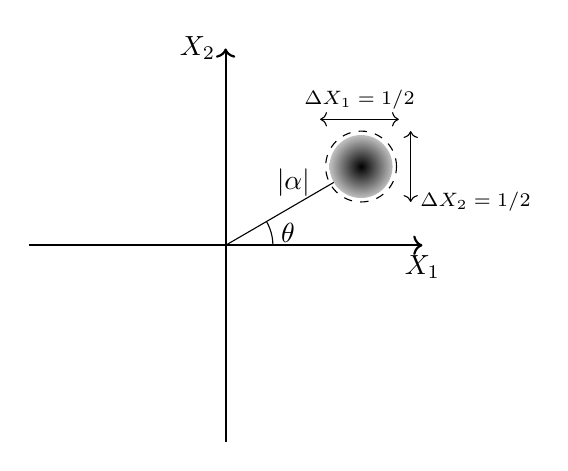
\begin{tikzpicture}
        \draw[thick,->] (-2.5,0) -- (2.5,0) node[anchor=north] {$X_1$};
        \draw[thick,->] (0,-2.5) -- (0,2.5) node[anchor=east] {$X_2$};
        \draw (0,0) -- (1.72,1) node[midway,anchor=south] {$|\alpha|$};
        \draw[dashed] (1.72,1) circle (0.45cm);
        \shade[inner color=black,outer color=lightgray] (1.72,1) circle (0.4cm);
        \draw (0.6,0) arc (0:30:0.6cm) node[midway,anchor=west] {$\theta$};
        \draw[<->] (2.35,0.55) node[anchor=west] {\scriptsize $\Delta X_2 = 1/2$} -- (2.35,1.45);
        \draw[<->] (1.2,1.6) -- (2.2,1.6) node[anchor=south,midway] {\scriptsize $\Delta X_1 = 1/2$};
    \end{tikzpicture}
    \caption{Quantum HO}
\end{figure}
\end{multicols}
How does the vacuum state look in this picture?
\begin{align}
    \langle(\Delta\xo)^2\rangle\langle(\Delta\xt)^2\rangle &\geq \frac{1}{16}
\end{align}
So if you make one of these smaller than $\frac14$, you can satisfy this equation by making the other larger - this forms squeezed states.
You can also squeeze the vacuum state.
\begin{multicols}{2}
\begin{figure}[H]
    \centering
    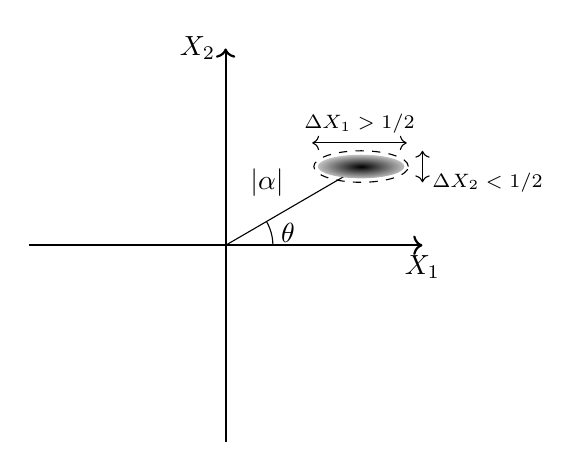
\begin{tikzpicture}
        \draw[thick,->] (-2.5,0) -- (2.5,0) node[anchor=north] {$X_1$};
        \draw[thick,->] (0,-2.5) -- (0,2.5) node[anchor=east] {$X_2$};
        \draw (0,0) -- (1.72,1) node[midway,anchor=south east] {$|\alpha|$};
        \draw[dashed] (1.72,1) ellipse (0.6cm and 0.2cm);
        \shade[inner color=black,outer color=lightgray] (1.72,1) ellipse (0.55cm and 0.15cm);
        \draw (0.6,0) arc (0:30:0.6cm) node[midway,anchor=west] {$\theta$};
        \draw[<->] (2.5,0.8) node[anchor=west] {\scriptsize $\Delta X_2 < 1/2$} -- (2.5,1.2);
        \draw[<->] (1.1,1.3) -- (2.3,1.3) node[anchor=south,midway] {\scriptsize $\Delta X_1 > 1/2$};
    \end{tikzpicture}
    \caption{Squeezed quadrature state}
\end{figure}
\begin{figure}[H]
    \centering
    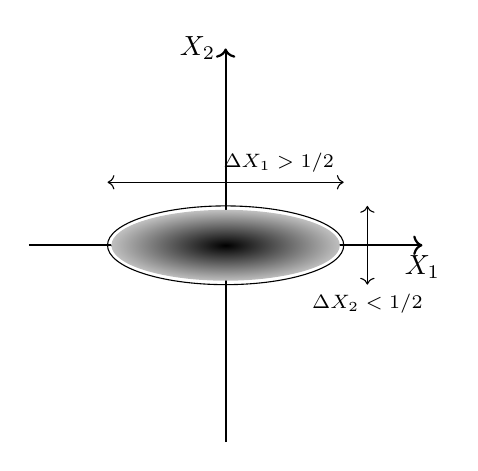
\begin{tikzpicture}
        \draw[thick,->] (-2.5,0) -- (2.5,0) node[anchor=north] {$X_1$};
        \draw[thick,->] (0,-2.5) -- (0,2.5) node[anchor=east] {$X_2$};
        \draw (0,0) ellipse (1.5cm and 0.5cm);
        \shade[inner color=black,outer color=lightgray] (0,0) ellipse (1.45cm and 0.45cm);
        \draw[<->] (1.8,-0.5) node[anchor=north] {\scriptsize $\Delta X_2 < 1/2$} -- (1.8,0.5);
        \draw[<->] (-1.5,0.8) -- (1.5,0.8) node[anchor=south east] {\scriptsize $\Delta X_1 > 1/2$};
    \end{tikzpicture}
    \caption{Squeezed vacuum state}
\end{figure}
\end{multicols}
You can squeeze the amplitude and make the phase more uncertain by showing the ellipse at an angle:
\begin{figure}[H]
    \centering
    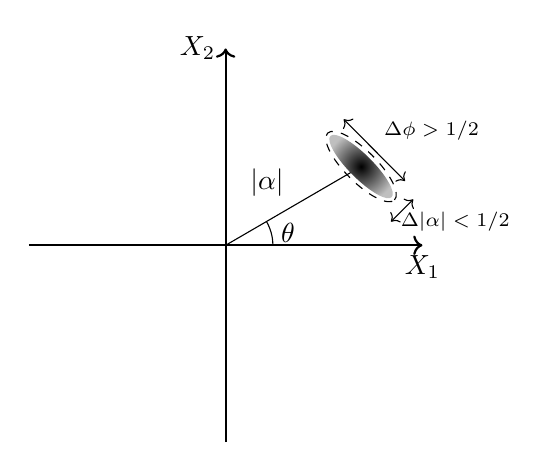
\begin{tikzpicture}
        \draw[thick,->] (-2.5,0) -- (2.5,0) node[anchor=north] {$X_1$};
        \draw[thick,->] (0,-2.5) -- (0,2.5) node[anchor=east] {$X_2$};
        \draw (0,0) -- (1.72,1) node[midway,anchor=south east] {$|\alpha|$};
        \draw[dashed,rotate around={-45:(1.72,1)}] (1.72,1) ellipse (0.6cm and 0.2cm);
        \shade[inner color=black,outer color=lightgray,rotate around={-45:(1.72,1)}] (1.72,1) ellipse (0.55cm and 0.15cm);
        \draw (0.6,0) arc (0:30:0.6cm) node[midway,anchor=west] {$\theta$};
        \draw[<->,rotate around={45:(2.1,0.3)}] (2.1,0.3) node[anchor=west] {\scriptsize $\Delta |\alpha| < 1/2$} -- (2.5,0.3);
        \draw[<->,rotate around={-130:(1.5,1.6)}] (1.5,1.6) -- (1.6,2.7) node[anchor=south west,midway] {\scriptsize $\Delta \phi > 1/2$};
    \end{tikzpicture}
    \caption{Squeezed phase state}
\end{figure}
To create these states, you need a new operator:
\begin{align}
    \hat{s}(\e) &= \exp\left[\frac12\left(\e^*\ha^2 - \e(\hag)^2\right)\right]
\end{align}
You can create this operator using:
\begin{itemize}
    \item non-linear crystals
    \item atomic gases
    \item 4-wave mixing
\end{itemize}
\begin{align}
    \hh &= \underbrace{\hbar\om\hag\ha}_{\text{signal mode}} + \underbrace{\hbar\om_p\hat{b}^\dagger\hat{b}}_{\text{pump mode}} + i\hbar\chi^{(2)}\left(\ha^2\hat{b}^\dagger - (\hag)^2\hat{b}\right)
\end{align}
$\chi^{(2)}$ is known as the second order non-linear susceptibility.
So we will treat the pump mode as almost classical,
\begin{align}
    \hat{b} &\to \beta e^{i\om_p t} & \hat{b}^\dagger &\to \beta^*e^{-i\om_p t} & \eta &= \chi^{(2)}\beta
\end{align}
From this, we can write our Hamiltonian in the parametric approximation:
\begin{align}
    \hh^{(PA)} &= \hbar\om\hag\ha + i\hbar\left(\eta^*\ha^2e^{i\om_p t} - \eta(\hag)^2e^{-i\om_p t}\right)
\end{align}
Then in the interaction picture,
\begin{align}
    \hh_{int} &= i\hbar\left(\eta^*\ha^2e^{i(\om_p - 2\om)t} - h.c.\right) \\
              &= i\hbar\left(\eta^*\ha^2 - \eta(\hag)^2\right),~ \om_p = 2\om \\
    U &= \exp\left(-\frac{i}{\hbar}\hh_{int}\right) = \exp\left(\eta^*\ha^2 - \eta(\hag)^2 \right)
\end{align}

\chapter{}
\section{Learning Outcomes}
Atom-light interaction and a model for photodetection.
We will develop a fully quantum mechanical model for the interaction of light with atoms. 
After studying this part, you should:
\begin{itemize}
    \item Be familiar with the atom-light interaction Hamiltonian in the electric dipole approximation, and explain this approximation.
    \item Be familiar with the Pauli operators asa quantum description of the two-level atom.
    \item Explain the physical basis of the Jaynes-Cummings model for atom-light interactions. Explain and use, but not derive, the resulting Hamiltonian.
    \item Be familiar with the concept of dressed state, and vacuum Rabi splitting in the context of the Jaynes Cummings Hamiltonian.
    \item Be able to perform simple calculations with combinations of atomic and field operators.
    \item Provide a simple explanation of a photodetector in the context of quantum optics. 
    \item Be familiar with the operator expression for the photodetection probability, and understand the meaning of normal ordering in this context.
\end{itemize}

\section{Atom-Light Interactions}
\begin{align}
    \hh &= \hh_{atom} + \hh_{field} + \hh_{int} \\
    \hh_{atom} &= \frac{\hp^2}{2m} + \hat{V}(r) 
\end{align}
So for the EM field, classical version in something of $\hat{A}$.
Interaction: force on $e^-$ due to EM field,
\begin{align}
    \unl{F} &- q\left[\E(\vr,t) + \unl{v}\times\B(\vr,t)\right]
\end{align}
where $\unl{F}$ is the Lorentz force. \textit{We do not need to know the derivation for this, only to use it.}
This is known as the minimal coupling Hamiltonian. 
Choose Coulomb gauge, $\phi=0,\,\del\cdot A = 0$, but note that this is not Lorentz invariant.
Now we apply the electric dipole approximation, where light $\gg$ atoms.
\begin{align}
    A_{\unl{k},s}(\vr,t) &= A_{\unl{k},s}\exp\left[i(\unl{k}\cdot\vr 0 \om_kt)\right] + c.c.
\end{align}
The length scale of the light in this is given by the wavevector, $\approx |\unl{k}| = 2\pi/\lambda$.
For visible light, $\lambda \approx 400-700\,nm$; for microwaves, $\lambda \approx 1\,cm$.
But for atoms, $\approx 0.1\,nm$, so as far as atoms are concerned, photons are huge.
If $\vr$ is the size of the atom, $\unl{k}\cdot\vr \ll 1$.
So $A(\vr,t) \approx A(t)$ over the size of the atom.
\begin{align}
    \hh_{int} &= e\hat{\vr}\cdot\Eh(t)
\end{align}
The sign of $e$ is positive, so $e^-$ is $-e$.
$e\hat{\vr} = \hat{\unl{d}}$, the electric dipole operator.
\begin{align}
    \hh_{int} &= \hat{\unl{d}}\cdot\Eh(t)
\end{align}
So we want a single mode field, and the best way to think about this is place the light into a cavity.
\begin{figure}
    \centering
    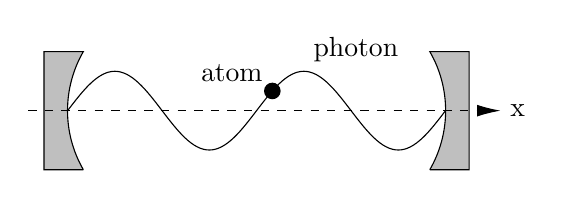
\begin{tikzpicture}
    \filldraw[fill=lightgray,draw=black] (0,0) -- (-0.5,0) -- (-0.5,1.5) -- (0,1.5) arc (150:210:1.5cm);
    \filldraw[fill=lightgray,draw=black] (4.4,0) -- (4.9,0) -- (4.9,1.5) -- (4.4,1.5) arc (30:-30:1.5cm);
    \draw (-0.2,0.75) sin (0.4,1.25) cos (1,0.75) sin (1.6,0.25) cos (2.2,0.75) sin (2.8,1.25) node[anchor=south west] {photon} cos (3.4,0.75) sin (4,0.25) cos (4.6,0.75);
    \draw[dashed,-{Latex[length=3mm,width=1.5mm]}] (-0.7,0.75) -- (5.3,0.75) node[anchor=west] {x};
    \fill (2.4,1) circle (3pt) node[anchor=south east] {atom};
    \end{tikzpicture}
\end{figure}
\begin{align}
    \Eh &= e_{\unl{k}}\left(\frac{\hbar\om_k}{\e_0V}\right)^{1/2}(\ha+\hag)\sin(kx)
\end{align}
Two level atom - the two that match EM field.
\begin{align}
    \hh &= \hh_{atom} + \hh_{field} + \hh_{int} \\
    \hh_{field} &= \hbar\left(\hag\ha + \frac12\right)
\end{align}
The $\frac12$ is the zero-point energy. 
A two-level atom is equivalent to a spin-$\frac12$ particle.
\begin{align}
    \hsig_+ &= |e\rangle\langle g| & \hsig_- &= |g\rangle\langle e| = \hsig^\dagger_+ \\
    \hsig_z &= |e\rangle\langle e| - |g\rangle\langle g| \\
    \hsig_+ &= \hsig_x + i\hsig_y & \hsig_- &= \hsig_x - \hsig_y
\end{align}
Now we can write the Hamiltonian for the atom:
\begin{align}
    \hh_{atom} &= \frac12(E_e - E_g)\hsig_z = \frac12\hbar\om_0\hsig_z \\
    \hh_{int} &= -\hd\cdot\Eh = g\hat{d}(\ha+\hag) \\
    g &= -\left(\frac{\hbar\om}{\e_0V}\right)^{1/2}\sin(kx) \\
    \langle g|\hd|g\rangle &= \langle e|\hd|e\rangle = 0 \\
    \hd &= d|g\rangle\langle e| + d^*|e\rangle\langle g| \\
        &= d(\hsig_+ + \hsig_-) \\
    \hh_{int} &= \hbar\left(\frac{dg}{\hbar}\right)(\hsig_+ +\hsig_-)(\ha+\hag) \\
    \hh &= \frac12\hbar\om_0\hsig_z + \hbar\om_k\left(\hag\ha+\frac12\right) + \hbar\lambda(\hsig_+ +\hsig_-)(\ha+\hag)
\end{align}
Note that $\lambda$ here is \unl{not a wavelength} but just the constant from Eq (7.19).

\section{Rotating Wave Approximation}
So in the Heisenberg picture, we have
\begin{align}
    \ha(t) &= \ha(0)e^{-i\om t} & \hag(t) &= \hag(0)e^{+i\om t} \\
    \hsig_+(t) &= \hsig_+(0)e^{+i\om_0t} & \hsig_-(t) &= \hsig_-(0)e^{-i\om_0 t} 
\end{align}
$\hh_{int}$ has:
\begin{align}
    \hsig_+\ha &\approx e^{i(\om_0-\om)t} & \hsig_-\hag &\approx e^{i(w-\om_0)t} \\
    \hsig_+\hag &\approx e^{i(\om+\om_0)t} & \hsig_-\ha &\approx e^{-i(\om+\om_0)t}
\end{align}
Eqs (7.23) oscillate slowly and conserve energy, while Eqs (7.24) oscillate fast and do not conserve energy.
So we want to drop the fast oscillating terms as these are not useful to our picture of the Hamiltonian, and this is the rotating wave approximation. 
From this, we arrive at the Jaynes-Cummings Hamiltonian:
\begin{align}
    \hh_{JC} &= \frac12\hbar\om_0\hsig_z + \hbar\om\left(\hag\ha+\frac12\right) + \hbar\lambda(\hsig_+\ha +\hsig_-\hag)
\end{align}
This describes: 
\begin{itemize}
    \item energy of atom
    \item energy of photons/cavity mode (single mode)
    \item how energy can be exchanged between atom and cavity mode
\end{itemize}
\begin{align}
    \hsig_+\ha|g\rangle|n\rangle &\implies |e\rangle|n-1\rangle \\
    \hsig_-\hag|e\rangle|n\rangle &\implies |g\rangle|n+1\rangle
\end{align}
\begin{multicols}{2}
So these behave like raising and lowering operators as they shift the atom around the cavity.\\
So what assumptions did we use?
\begin{itemize}
    \item electron can't go anywhere else outside the cavity
    \item number of photons is fixed, such that there were no other losses to outside the cavity
    \item only need $|g\rangle,|e\rangle$ for the two levels of the atom and $|n\rangle,|n+1\rangle$ for the states of the photons
\end{itemize}
\columnbreak
\begin{figure}[H]
    \centering
    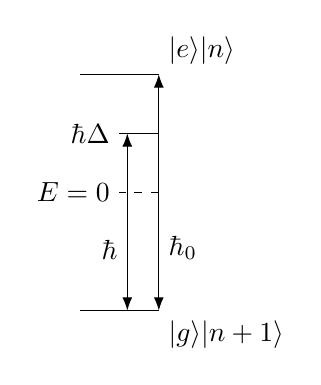
\begin{tikzpicture}
        \draw (0,0) -- (1,0) node[anchor=north west] {$|g\rangle|n+1\rangle$};
        \draw (0,3) -- (1,3) node[anchor=south west] {$|e\rangle|n\rangle$};
        \draw[Latex-Latex] (1,3) -- (1,0) node[anchor=west,midway,yshift=-20pt] {$\hbar\om_0$};
        \draw[dashed] (1,1.5) -- (0.5,1.5) node[anchor=east] {$E=0$}; 
        \draw (1,2.25) -- (0.5,2.25) node[anchor=east] {$\hbar\Delta$};
        \draw[Latex-Latex] (0.6,2.25) -- (0.6,0) node[anchor=east,midway,yshift=-10pt] {$\hbar\om$};
    \end{tikzpicture}
\end{figure}
\end{multicols}
We can then form two basis states:
\begin{align}
    |\psi_1,n\rangle &\equiv |e\rangle|n\rangle = |i\rangle & |\psi_2,n\rangle &\equiv |g\rangle|n+1\rangle = |f\rangle
\end{align}
\begin{equation}
    \hh(n) = \hbar\begin{pmatrix} n\om+\frac12\om_0 & \lambda\sqrt{n+1} \\ \lambda\sqrt{n+1} & (n+1)\om-\frac12\om_0\end{pmatrix}
\end{equation}
Matrix elements obtained from $\langle i|\hh(n)|i\rangle$, etc.

\chapter{}
\section{Rotating Wave Approx Ctd}
We will take $\Delta=0$, and for an initial state $|i\rangle = |e\rangle|n\rangle$,
\begin{align}
    |\psi(t)\rangle &= c_i(t)|i\rangle + c_f(t)|f\rangle \\
    E_i &= \frac12\hbar\om + n\hbar\om,~ E_f = -\frac12\hbar\om + (n+1)\hbar\om
\end{align}
So the energies are equal, and conserved.
We can then solve the Schrodinger equation for Eq (8.1), and find relations for the co-factors:
\begin{align}
    \dot{c}_i &= -i\lambda\sqrt{n+1}c_f & \ddot{c}_i &+ \lambda^2(n+1)c_i = 0 \\
    c_i(t) &= \cos\left(\lambda t\sqrt{n+1}\right) & c_f(t) &= i\sin\left(\lambda t\sqrt{n+1}\right) 
\end{align}
\begin{equation}
    P_i(t) = |c_i(t)|^2 = \cos^2\left(\lambda t\sqrt{n+1}\right)
\end{equation}
To figure this out, we can go through many different solutions, but the simplest in this problem is to use what is called the \textbf{atomic inversion}:
\begin{align}
    \om(t) &= \langle\psi(t)|\hsig_z|\psi(t)\rangle \\
           &= P_i(t) - P_f(t) = \cos\left(2\lambda t\sqrt{n+1}\right)
\end{align}
Now we will define the \textbf{Rabi frequency}, as
\begin{align}
    \Om(n) &= 2\lambda\sqrt{n+1}
\end{align}
Note that there are even Rabi oscillations for $n=0$.
This may seem a strange possibility at first, but there are many experiments to prove this is in fact the case, where it occurs in our cavity model as the vacuum of the single mode focused on the atom. 
This can appear quite classical at first, but in the more general case as you increase the number of states involved, it will seem more quantum.
We can write general descriptions for our ground and excited states:
\begin{align}
    |\psi_g(t)\rangle &= -i\sin_{n=0}^\infty c_n\sin\left(\frac12\Om(n)\right)|n+1\rangle \\
    |\psi_e(t)\rangle &= \sum_{n=0}^\infty c_n\cos\left(\frac12\Om(n)t\right)|n\rangle \\
    \om(t) &= \sum_{n=0}^\infty |c_n|^2\cos\left(\Om(n)t\right),\; c_n = \frac{\alpha^n}{\sqrt{n!}}e^{-|\alpha|^2/2}
\end{align}
For a single number state, $P_i$ oscillates between ground and excited in a classical sinusoidal appearance, but when we consider a coherent state with average $\langle n\rangle$, it drops down into being a superposition of being ground and excited, then after a while excites into partial oscillations again, and continues this interesting pattern.
\textit{input graphs}

Now, we want to analyse the Jaynes-Cummings Hamiltonian through the calculation of the matrix elements instead, so we will start with our same two pairs of states, this time with $\Delta\neq0$.
\begin{align}
    |i\rangle &= |e\rangle|n\rangle & |f\rangle &= |g\rangle|n+1\rangle 
\end{align}
\begin{equation}
    \hh(n) = \hbar\begin{pmatrix}n\om+\frac12\om_0 & \lambda\sqrt{n+1} \\ \lambda\sqrt{n+1} & (n+1)\om-\frac12\om_0 \end{pmatrix}
\end{equation}
This has eigenenergies with the Rabi frequency, which is the same as before if $\Delta=0$.
\begin{align}
    E_{\pm} &= \hbar\left\{\left(n+\frac12\right)\om \pm \frac12\Om_n(\Delta)\right\} \\
    \Om_n(\Delta) &= \left[\Delta^2+ 4\lambda^2(n+1)\right]^{1/2} 
\end{align}
We then have eigenstates, 
\begin{align}
    |n,+\rangle &= \cos\left(\frac12\Phi_n\right)|i\rangle + \sin\left(\frac12\Phi_n\right)|f\rangle & |n,-\rangle &= -\sin\left(\frac12\Phi_n\right)|i\rangle + \cos\left(\frac12\Phi_n\right)|f\rangle
\end{align}
We have used a new angle here, $\Phi_n$, where this is defined as
\begin{align}
    \Phi_n &= \arctan\left(\frac{2\lambda\sqrt{n+1}}{\Delta}\right) = \arctan\left(\frac{\Om_n(0)}{\Delta}\right).
\end{align}
We are happy with this definition even in the limit of $\Delta\to0$, as $\tan$s have known angles even at $\infty$.\\
The eigenstates above are known as \emph{dressed states} of the atom, so when the atom is in a single-mode field like this, the field changes the eigenstates so they become eigenstates of the whole system. 
This looks like the energies of the eigenstates being changed by the application of the field.
The original eigenstates we considered, $|e\rangle|n\rangle$ and $|g\rangle|n+1\rangle$, are called \emph{bare states.}
These bare states do not have the same energy, unless $\Delta=0$.
\begin{figure}[H]
    \centering
    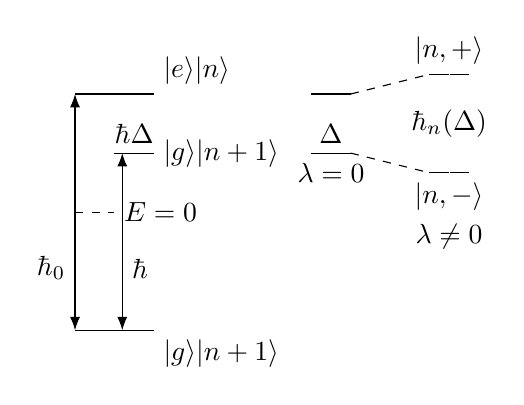
\begin{tikzpicture}
        \draw (0,0) -- (1,0) node[anchor=north west] {$|g\rangle|n+1\rangle$};
        \draw (0,3) -- (1,3) node[anchor=south west] {$|e\rangle|n\rangle$};
        \draw[Latex-Latex] (0,3) -- (0,0) node[anchor=east,midway,yshift=-20pt] {$\hbar\om_0$};
        \draw[dashed] (0,1.5) -- (0.5,1.5) node[anchor=west] {$E=0$}; 
        \draw (0.5,2.25) -- (1,2.25) node[anchor=south,midway] {$\hbar\Delta$} node[anchor=west] {$|g\rangle|n+1\rangle$};
        \draw[Latex-Latex] (0.6,2.25) -- (0.6,0) node[anchor=west,midway,yshift=-10pt] {$\hbar\om$};

        \draw (3,2.25) -- (3.5,2.25) node[anchor=south,midway] {$\Delta$} node[anchor=north,midway] {$\lambda=0$};
        \draw (3,3) -- (3.5,3);
        \draw[dashed] (3.5,2.25) -- (4.5,2);
        \draw (4.5,2) -- (5,2) node[anchor=north,midway] {$|n,-\rangle$} node[anchor=north,midway,yshift=-15pt] {$\lambda\neq0$}; 
        \draw[dashed] (3.5,3) -- (4.5,3.25);
        \draw (4.5,3.25) -- (5,3.25) node[anchor=south,midway] {$|n,+\rangle$};
        \draw[white] (4.75,3.25) -- (4.75,2) node[black,midway] {$\hbar\Om_n(\Delta)$};
    \end{tikzpicture}
\end{figure}
So if we define $\Delta=\om_0-\om$, we can see that now $\Delta$ is the energy splitting between the states $|e\rangle|n\rangle$ and $|g\rangle|n+1\rangle$, but this is for $\lambda=0$ and we can see the dependence on $\lambda$ on these energy states through the Rabi frequency. 
It is then clear that this energy splitting $\Delta$, will increase for the eigenenergies, $|n,-\rangle$ and $n,+\rangle$.
This is known as a \emph{Stark Shift}, since it is interacting through the E-field of light. 
Specifically, it is known as the AC or dynamic Stark shift, as the source of the electric field is not static, but dynamic.\\
So as $\Delta\to0$, we are on resonance, and the bare states are degenerate, but the dressed states are still split.
\begin{align}
    \arctan&\left(\frac{2\lambda\sqrt{n+1}}{\Delta\to0}\right) \to \frac{\pi}{2} & \cos\left(\frac12\Phi_n\right) &= \sin\left(\frac12\Phi_n\right) \to \frac{1}{\sqrt{2}} \\
    |n,+\rangle &= \frac{1}{\sqrt{2}}\left(|e\rangle|n\rangle+|g\rangle|n+1\rangle\right) & |n,-\rangle &= \frac{1}{\sqrt{2}}\left(-|e\rangle|n\rangle+|g\rangle|n+1\rangle\right)
\end{align}
\begin{figure}[H]
    \centering
    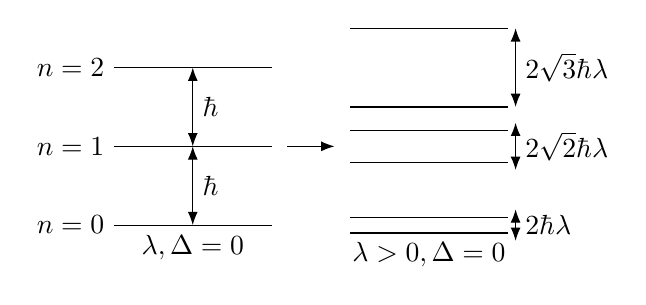
\begin{tikzpicture}
        \draw (0,0) node[anchor=east] {$n=0$} -- (2,0) node[anchor=north,midway] {$\lambda,\Delta=0$}; 
        \draw (0,1) node[anchor=east] {$n=1$} -- (2,1);
        \draw (0,2) node[anchor=east] {$n=2$} -- (2,2);
        \draw[Latex-Latex] (1,0) -- (1,1) node[anchor=west,midway] {$\hbar\om$};
        \draw[Latex-Latex] (1,1) -- (1,2) node[anchor=west,midway] {$\hbar\om$};

        \draw[-Latex] (2.2,1) -- (2.8,1);

        \draw (3,-0.1) -- (5,-0.1) node[anchor=north,midway] {$\lambda>0,\Delta=0$};
        \draw (3,0.1) -- (5,0.1);
        \draw[Latex-Latex] (5.1,-0.2) -- (5.1,0.2) node[anchor=west,midway] {$2\hbar\lambda$};
        \draw (3,0.8) -- (5,0.8);
        \draw (3,1.2) -- (5,1.2);
        \draw[Latex-Latex] (5.1,0.7) -- (5.1,1.3) node[anchor=west,midway] {$2\sqrt{2}\hbar\lambda$};
        \draw (3,1.5) -- (5,1.5);
        \draw (3,2.5) -- (5,2.5);
        \draw[Latex-Latex] (5.1,1.5) -- (5.1,2.5) node[anchor=west,midway] {$2\sqrt{3}\hbar\lambda$};
    \end{tikzpicture}
\end{figure}
The phenomenom shown above is known as vacuum Rabi splitting, where we get anharmonic energy levels due to coupling as $\lambda\neq0$.
This is the underlying physics that allows us to engineer quantum technology by compressing waves down several orders of magnitude.
This all begins as the light and atom when allowed to interact begin to behave as a composite system.

\chapter{}
\section{Photodetection}
We are interested in detecting low numbers of photons, so we will make use of the physics previously discussed, in terms of Hamiltonians
\begin{align}
    \hh &= \hh_{field} + \hh_{atom} + \hh_{int} \\
    \hh_{field} &= \sum_{\unl{k},s}\hbar\om_k\left(\hag_{\unl{k},s}\ha_{\unl{k},s}+\frac12\right) \\
    \hh_{atom} &= \hbar\om_0\hsig_z,\; |k| = \frac{2\pi}{\lambda} \\
\end{align}
We then want to use the electric dipole approximation to build our interaction Hamiltonian,
\begin{align}
    \hh_{int} &= e\hat{\vr}\cdot\Eh = -\hat{d}\cdot\Eh(\vec{R},t)
\end{align}
We are aiming to ionise the atom, because then we have a free electron to detect as well. 
Once we have one electron freed, we can pull many more until we have multiple electrons to form a current, which we can detect.
Of course to ionise the atom, we require the photon to add enough energy to free the electron.

Two types of photodetectors:
\begin{itemize}
    \item Photomultiplier tube (PMT):
        \textit{draw doodle, photo multiplier tube, photon bumps into cathode, then e bumps into next, etc etc, the first is a cathode, then lots of dynodes, then an anode attached to a resistor to detect the current.}
        It is in a tube so it has a high vacuum. 
        This tube can result in a gain $\approx 10^8$.
    \item Avalanche Photo Detecto (APD)
        \textit{draw doodle, see notes}
        We do not have as high a gain here, but using a semiconductor instead of a high vacuum is more practical and easier to make.
\end{itemize}
\textit{more doodles}
For a free electron, 
\begin{align}
    |e\rangle &= \frac{1}{\sqrt{V}}e^{i\vec{q}\cdot\vr}
\end{align}
So for our interaction Hamiltonian then, 
\begin{align}
    \hh_{int} &= -\hat{d}\cdot\Eh(\vr,t) \\
    \Eh(\vr,t) &= i\sum_{\unl{k},s}\left(\frac{\hbar\om_k}{2\e_0V}\right)^{1/2}\ve_{\unl{k},s}\left[\hag_{\unl{k},s}(t)e^{i\unl{k}\cdot\vr} - \ha_{\unl{k},s}(t)e^{-i\unl{k}\cdot\vr}\right]
\end{align}
This is clearly in the Heisenberg picture as we have time-dependent operators. 
Here, $\ve$ is the polarisation vector.
\begin{align}
    \ha_{\unl{k},s}(t) &= \ha_{\unl{k},s}e^{-i\om_kt} & \hag_{\unl{k},s}(t) &= \hag_{\unl{k},s}e^{i\om_kt}
\end{align}
We want to split the electric field into two parts for absorption and emission:
\begin{align}
    \Eh_+(\vr,t) &\equiv i\sum_{\unl{k},s}\left(\frac{\hbar\om_k}{2\e_0V}\right)^{1/2}\ve_{\unl{k},s}\ha_{\unl{k},s}(t)e^{i\vec{k}\cdot\vr} \\
    \Eh_-(\vr,t) &\equiv -i\sum_{\unl{k},s}\left(\frac{\hbar\om_k}{2\e_0V}\right)^{1/2}\ve_{\unl{k},s}\hag_{\unl{k},s}(t)e^{-i\vec{k}\cdot\vr} \\
\end{align}
These have been defined such that $\Eh_- \equiv \Eh_+^\dagger$ and vice versa; these operators have taken on the properties of the creation and annihilation operators. 
We only want to use $\Eh_+$ as this deals with absorption, which is what we're interested in. 
\begin{align}
    \langle F|\hh|I\rangle &\approx -\underbrace{\langle e|\hat{d}|g\rangle}_{\text{atom}} \underbrace{\langle f|\Eh_+(\vr,t)|i\rangle}_{\text{field}} 
\end{align}
The atom term above is equal to $d$, but the field term isn't so clear. 
We must sum over all possible final states to find this expectation value, using the \textbf{broadband detector assumption.}
\begin{align}
    P_f &= |\langle F|\hh|I\rangle|^2 \propto |\langle f|\Eh_+(\vr,t)|i\rangle|^2 \\
    P_i &\propto \sum_f |\langle f|\Eh_+(\vr,t)|i\rangle|^2 \\
        &\propto \sum_f \langle i|\Eh_-(\vr,t)|f\rangle\langle f|\Eh_+(\vr,t)|i\rangle
\end{align}
If this sum is over all possible $f$ and doesn't depend on any of the other terms, then the $|f\rangle\langle f|$ will sum to the identity.
\begin{align}
    P_i &\propto \langle i|\Eh_-(\vr,t)\Eh_+(\vr,t)|i\rangle \\
    \Eh_+(\vr,t) &\equiv i\sum_{\unl{k},s}\left(\frac{\hbar\om_k}{2\e_0V}\right)^{1/2}\ve_{\unl{k},s}\ha_{\unl{k},s}(t)e^{i\vec{k}\cdot\vr} 
\end{align}
Depending on what our state is, wrapping it around the electric field operators can produce some fairly non-trivial outcomes.
Note that the ordering of these operators is important; if the operators were the other way around, they would be acting on the f bra/kets instead of the i bra/kets, and we would not have been able to sum and cancel the fs.\\
Reminding ourselves that we are trying to count photons, we can see that $\Eh_-\Eh_+ \propto \hag\ha = \hn$, the number operator. 
Therefore our current result makes sense as it will indeed count photons, for discrete states or coherent states (detecting average number of photons instead).
We will see more on this when we discuss correlation functions in lecture 11, but we first need to understand beamsplitters in lecture 10.

\section{Coherence/correlation functions}
First, we will remind ourselves of the classical functions. 
An early example is Young's slits experiment:
\textit{doodle}
We need 
\begin{align}
    \Delta s &\leq \frac{c}{\Delta\om} \\
    \Delta t &= \frac{\Delta s}{c} = \frac{1}{\Delta\om}
\end{align}
$\frac{c}{\Delta\om}$ is the coherence length, and $\Delta t$ is the coherence time.
Now what about the fiel at the detector?
\begin{align}
    t_1 &= t-\frac{s_1}{c},\; t_2 = t-\frac{s_2}{c} \\
    \E(\vr,t) &= k_1\E(\vr_1,t_1) + k_2\E(\vr_2,t_2) \\
    I(\vr) &= \langle |\E(\vr,t)|^2\rangle_t \\
           &= |k_1|^2\langle|\E(\vr_1,t_1)|^2\rangle + |k_2|^2\langle|\E(\vr_2,t)|^2\rangle + 2\text{Re}\left[k_1^*k_2\langle\E^*(\vr_1,t_1)\E(\vr_2,t_2)\rangle\right] \\
           &= I_1 + I_2 + 2\text{Re}[\text{interference}]
\end{align}
So we introduce $\gamma^{(1)}(x_1,x_2)$.
This is the first order normalised mutual coherence function. 
\begin{align}
    \gamma^{(1)}(x_1,x_2) &= \frac{\langle\E^*(\vr_1,t_1)\E(\vr_2,t_2)\rangle}{\left\{\langle|\E(\vr_1,t_1)|^2\rangle\langle|\E(\vr_2,t_2)|^2\rangle\right\}^{1/2}} \\
    I(\vr) &= I_1 + I_2 + 2\sqrt{I_1I_2}\text{Re}\left[k_1^*k_2\gamma^{(1)}(x_1,x_2)\right]
\end{align}
Now we set $k_j = |k_j|e^{i\phi_j}$.
\begin{align}
    I(\vr) &= I_1 + I_2 + 2\sqrt{I_1I_2}|\gamma^{(1)}(x_1,x_2)|\cos(\phi_1-\phi_2) \\
\end{align}
The $\cos$ term in this is the phase difference from path difference.
The value of $\gamma^{(1)}$ sets the amount of coherence: 
\begin{equation}
    \gamma^{(1)} \begin{cases} = 1 & \text{full coherence} \\ >0,\,<1 & \text{partial coherence} \\ = 0 & \text{no coherence}\end{cases}
\end{equation}


\end{document}


















